\documentclass[12pt,letterpaper]{article}

%\usepackage{times}
%\usepackage{epsfig}
\usepackage{graphicx}
%\usepackage{amsmath}
%\usepackage{amssymb}
\usepackage{hyperref}
\usepackage{tabularx}
\usepackage[left=1in, right=1in, top=1in, bottom=1in]{geometry}
\usepackage{titling}
\usepackage{setspace}
\usepackage{sectsty}
\usepackage{tabto}
\graphicspath{{../img/}} % adds the assets directory to the path, throw your images there
\usepackage{fancyhdr}
\pagestyle{fancy}
\fancyhf{}
\fancyheadoffset{0cm}
\renewcommand{\headrulewidth}{0pt} 
\renewcommand{\footrulewidth}{0pt}
\fancyhead[R]{\thepage}
\fancypagestyle{plain}{%
  \fancyhf{}%
  \fancyhead[R]{\thepage}%
}

\usepackage{cite}
\usepackage[sectionbib]{natbib}
\renewcommand{\refname}{}

\begin{document}
\fontfamily{ptm}\selectfont
\sectionfont{\fontsize{12}{12}\fontfamily{ptm}\selectfont}
\doublespacing
%%%%%%%%%%%%%%%%%%%%%%%%%%%%%% TITLE %%%%%%%%%%%%%%%%%%%%%%%%%%%%%%%%%%%%%%
\setlength{\droptitle}{1in} 

\title{\large{AN ABSTRACTED PYTHON CLASS FOR TDSP ML PROJECTS: \\ EXAMPLE USE CASE WITH WINE ID \\\vspace{1.2in}}}

\author{
Kevin Geidel \\
MSDS 422: Practical Machine Learning \\
Northwestern University \\
June 2, 2024 \\
}

\date{}
\maketitle
\thispagestyle{empty}	
\clearpage
\setcounter{page}{1}

%%%%%%%%%%%%%%%%%%%%%%%%%%%%%% PAGE 1 %%%%%%%%%%%%%%%%%%%%%%%%%%%%%%%%%%%%
\section{Executive summary}
\tab At some point ill cite this \citep{tdsp:2024} or even this \citep{Hyatt:2024}!!

\section{Research design}
\tab 
-Can we abstract datamining to automate model evaluation and selection?
-In a big MS thesis like data sync design where you use ORM youll want a custom pipeline toolkit 
-Wine defect prediction use case

\section{Exploratory Data Analysis (EDA)}
\tab 

\section{Datamining data models}

\section{Data pipeline and ML preprocessing}
\tab 

\section{ML engineering, evaluation and deployment}
\tab 
- data transformations!

\section{Findings}
\tab 

\section{Conclusions}
\tab 


\pagebreak
\section*{\center{Appendix}}


\begin{figure}[h!]
  \centering
    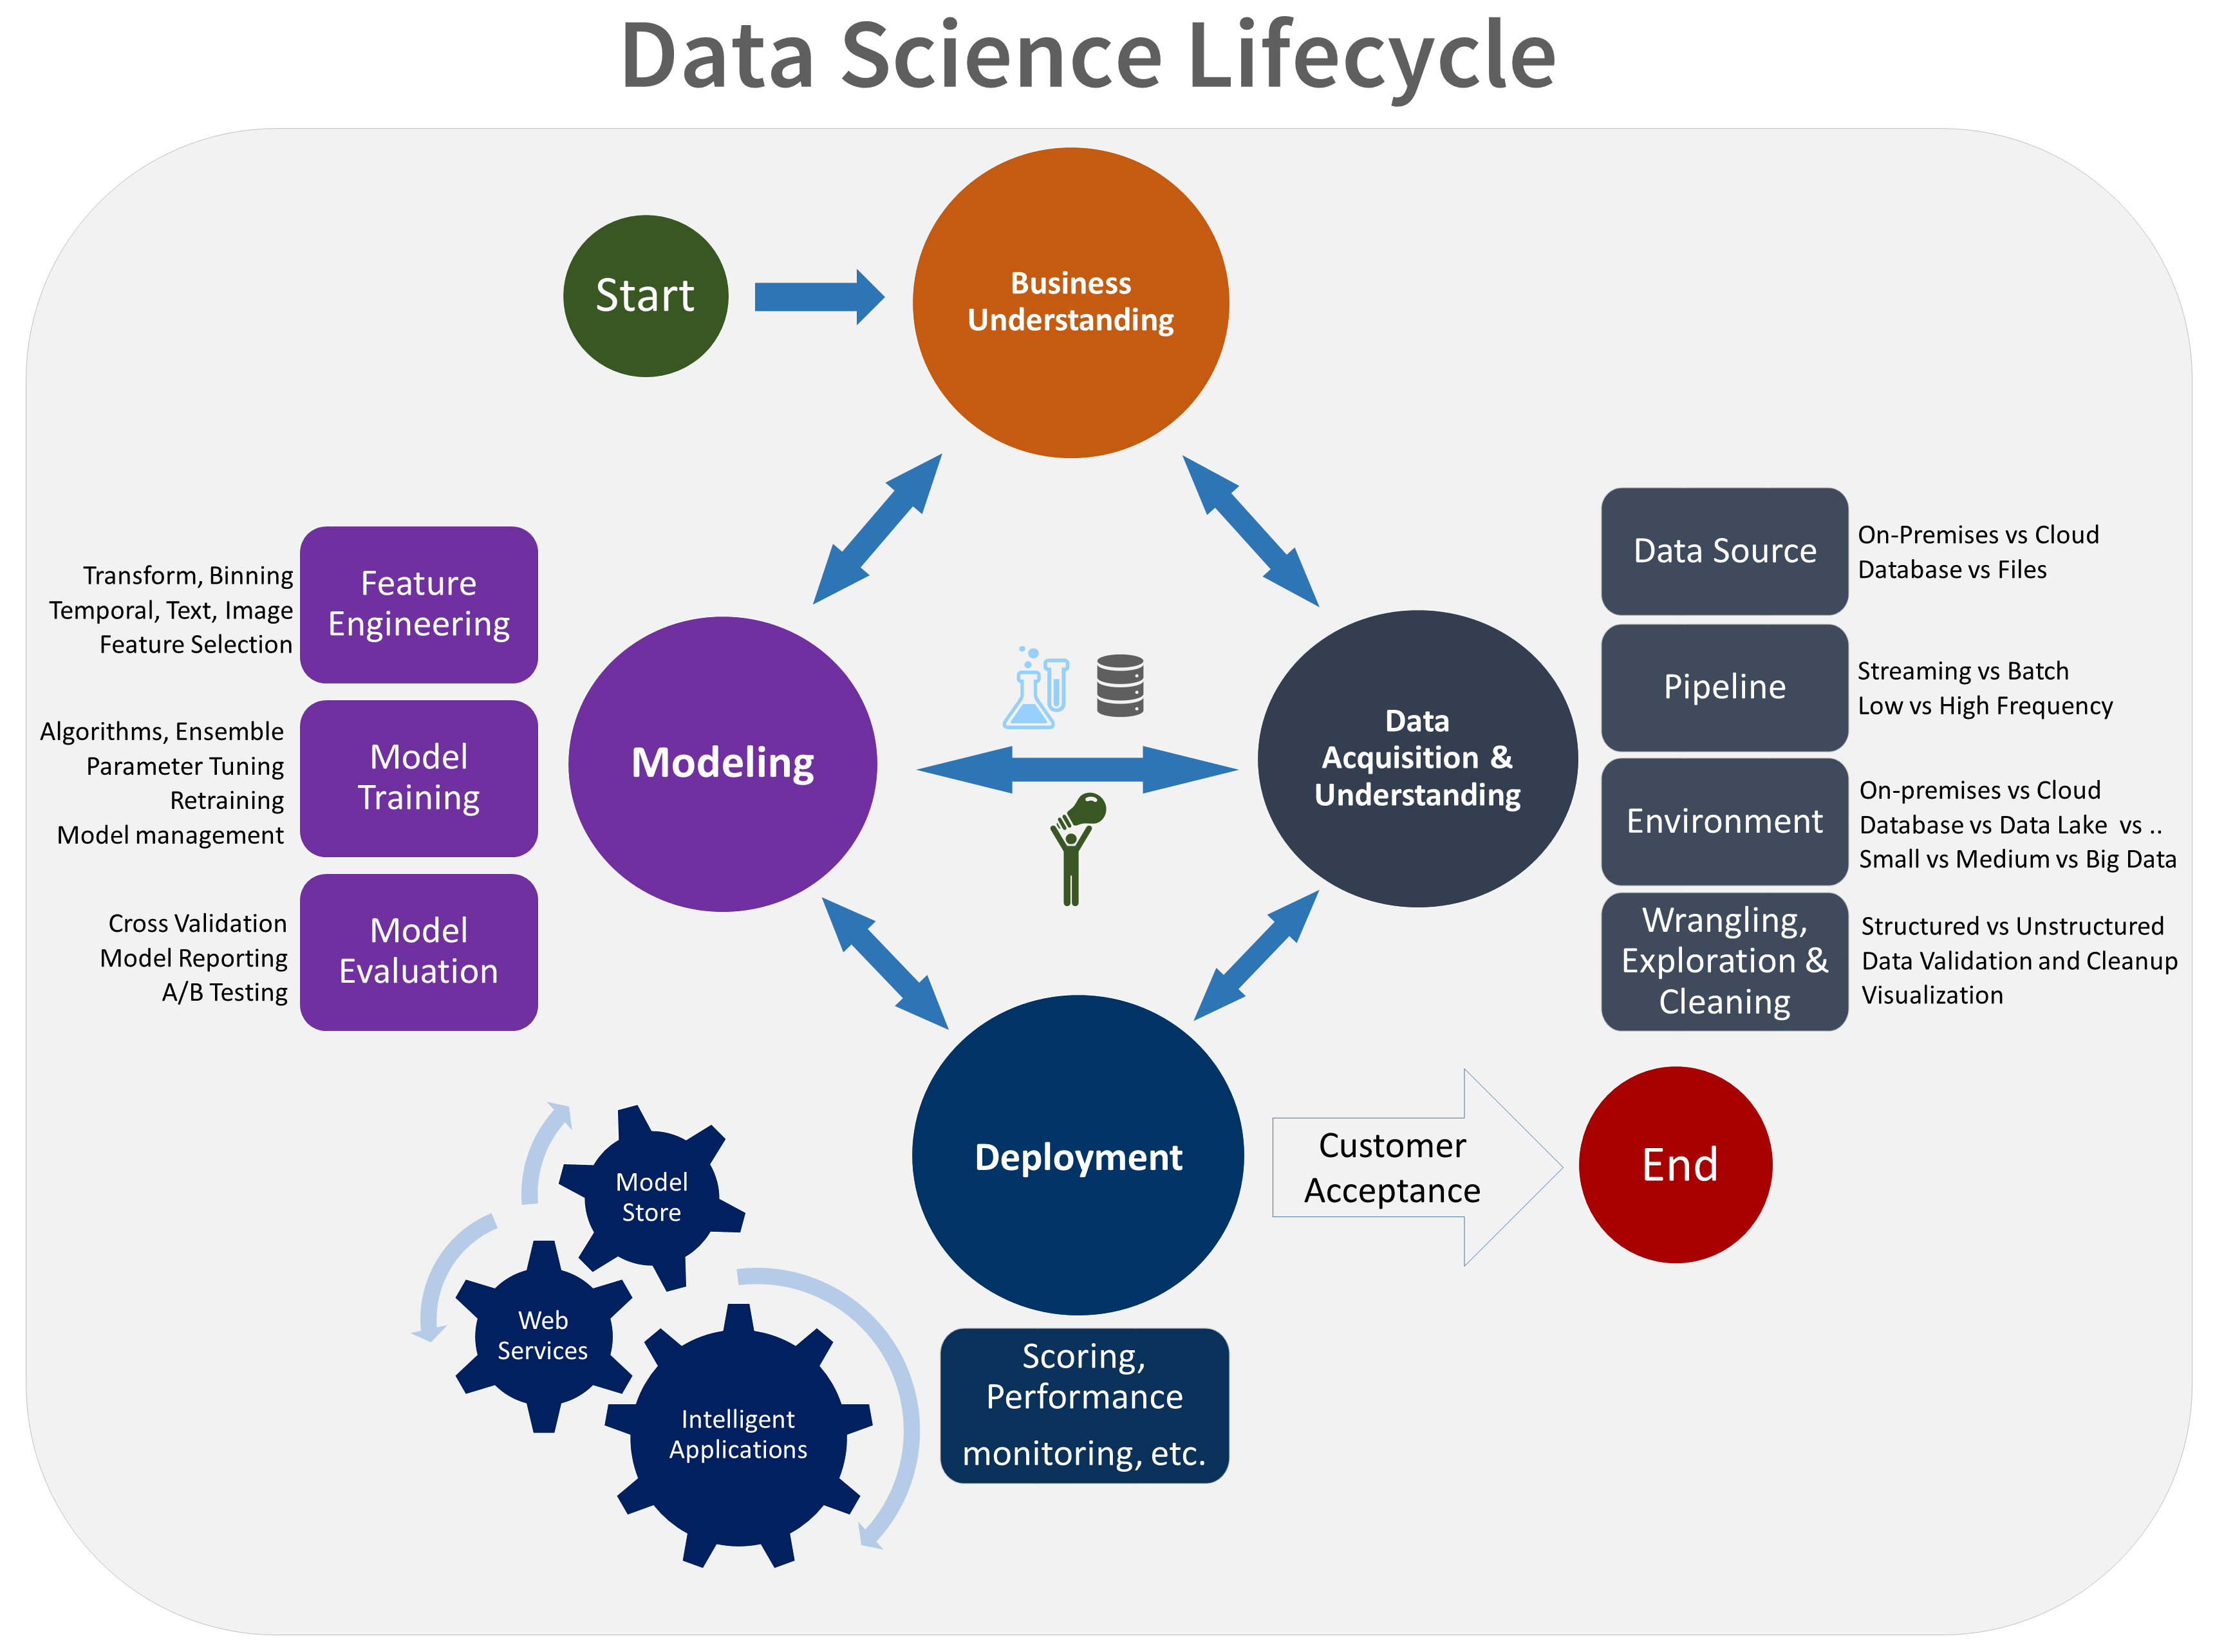
\includegraphics[width=1.0\linewidth]{../img/TDSP_Data_Science_Lifecycle.png}
    \caption{(color online) The ``data lifecycle'' in Team Data Science Process (TDSP)}
    \label{fig:tdsp}
  \end{figure}


\clearpage
\section*{\center{References}}
\bibliographystyle{chicago}
\center{\bibliography{references}}



\end{document}